\subsection{Performance evaluation of microservices communication with \acrshort{rest}, \acrshort{graphql}, and \acrshort{grpc} \cite{niswar_performance_2024}}
\label{sec:3-niswar}

A pesquisa de \textcite{niswar_performance_2024} propõe uma avaliação e comparação abrangente do desempenho de três protocolos de comunicação amplamente utilizados em arquiteturas de microsserviços: \gls{rest}, \acrshort{graphql} e \gls{grpc}. O estudo concentra-se na troca de dados, abordando cenários de recuperação de dados planos e aninhados, com o objetivo de fornecer insights valiosos para que desenvolvedores e arquitetos possam otimizar a escolha dos protocolos de comunicação, considerando casos de uso e cargas de trabalho específicas.

O desafio da comunicação eficiente entre esses serviços independentes é um ponto central do trabalho. Embora os autores apontem o \gls{rest} como o método mais popular para troca de dados, eles argumentam que este protocolo apresenta desvantagens, como o over-fetching (recuperação de mais dados do que o necessário) e o under-fetching (recuperação de dados insuficientes, o que exige requisições adicionais). Nesse contexto, o \acrshort{graphql} surge como uma alternativa para superar tais ineficiências, permitindo que os clientes especifiquem exatamente os dados necessários. Já o \gls{grpc}, segundo os autores, destaca-se por sua abordagem eficiente e versátil na comunicação entre serviços distribuídos, utilizando o protocolo \acrshort{http}/2, que suporta streaming de dados e simplifica chamadas de procedimento remoto em diversas linguagens de programação.

Para realizar a avaliação, os autores estabeleceram um ambiente experimental composto por três microsserviços implementados em contêineres, cada um com um banco de dados Redis para cache em memória e MySQL para armazenamento persistente. O estudo utilizou dados de um Sistema Integrado de Informação Educacional, focando especificamente nas informações sobre o perfil dos professores e em seus históricos educacionais, abrangendo dados planos e aninhados. A metodologia de avaliação de desempenho empregou o Apache JMeter\footnote{Disponível em \hyperref[https://jmeter.apache.org]{https://jmeter.apache.org}} para simular testes de carga de \gls{api}, coletando métricas-chave como tempo de resposta e utilização da CPU. Foram realizadas duas abordagens de avaliação: requisições concorrentes e requisições consecutivas, com o número de requisições variando de 100 a 500, a fim de simular diferentes níveis de carga, conforme \autoref{fig:2-niswar-1}.

\begin{figure}[H]
    \caption{Cenário proposto por \textcite{niswar_performance_2024}}
    \label{fig:2-niswar-1}
    \centering
    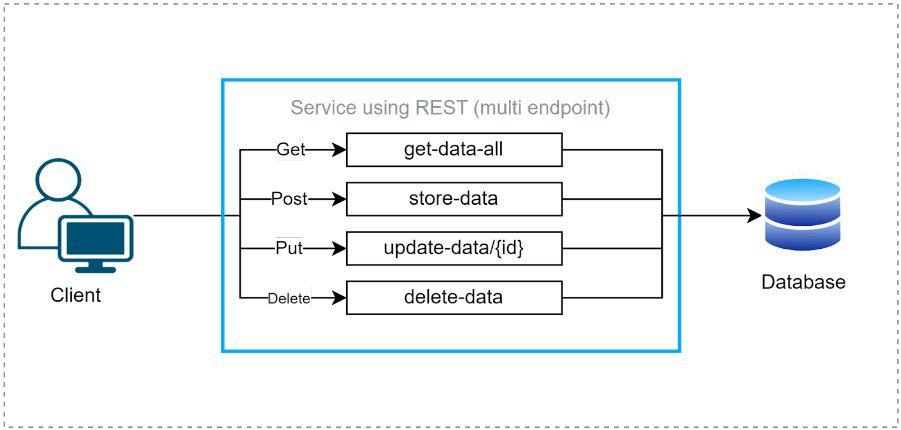
\includegraphics[width=0.75\linewidth]{imagens/niswar-1-enviroment.jpg}    
    {\par \raggedright \footnotesize Fonte: \textcite{niswar_performance_2024}.\par}
\end{figure}

Nos testes de requisições concorrentes, o tempo de resposta médio configurou-se como uma métrica crucial. Tanto para a recuperação de dados planos quanto aninhados, o \gls{grpc} demonstrou consistentemente tempos de resposta significativamente inferiores aos observados com \gls{rest} e \acrshort{graphql}. Por exemplo, para 100 requisições de dados planos, o \gls{grpc} foi aproximadamente 5 vezes mais rápido que o \gls{rest} e 16 vezes mais rápido que o \acrshort{graphql}. Essa vantagem de desempenho do \gls{grpc} manteve-se e intensificou-se à medida que o número de requisições aumentava, como pode ser observado nas figuras \ref{fig:2-niswar-time-flat} e \ref{fig:2-niswar-time-nested}.

Os resultados reforçam a eficiência do \gls{grpc} tanto para estruturas de dados simples quanto complexas e sob diferentes cargas, atribuída pelos autores ao uso do protocolo \acrshort{http}/2 e à serialização binária via Protocol Buffers.

\begin{figure}[htb]
  \centering
  \begin{minipage}[t]{0.48\linewidth}
    \caption{Tempos de respostas dos microsserviços com dados Flat}
    \label{fig:2-niswar-time-flat}
    \centering
    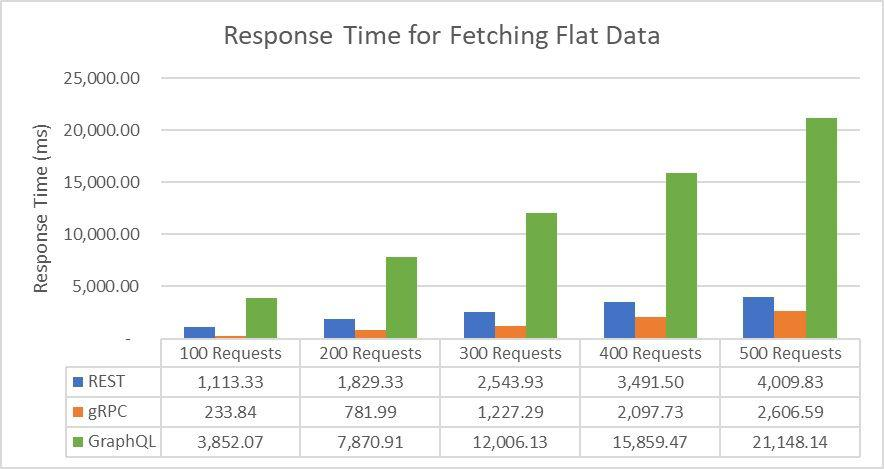
\includegraphics[width=\linewidth]{imagens/niswar_time_flat.jpg}    
    {\par \raggedright \footnotesize Fonte: \textcite{niswar_performance_2024}.\par}
  \end{minipage}%
  \hfill
  \begin{minipage}[t]{0.48\linewidth}
    \caption{Tempos de respostas dos microsserviços com dados Aninhados}
    \label{fig:2-niswar-time-nested}
    \centering
    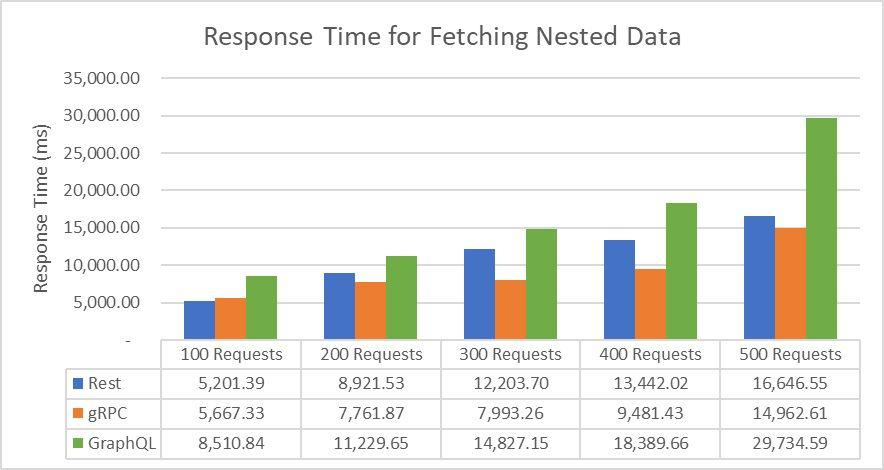
\includegraphics[width=\linewidth]{imagens/niswar_time_nested.jpg}    
    {\par \raggedright \footnotesize Fonte: \textcite{niswar_performance_2024}.\par}
  \end{minipage}
\end{figure}

Em relação à utilização da CPU, os resultados revelaram diferenças notáveis entre os protocolos, como ilustrado nas figuras \ref{fig:2-niswar-cpu-flat} e \ref{fig:2-niswar-cpu-nested}. Para a recuperação de dados planos, o protocolo \gls{rest} apresentou a menor utilização média da CPU, enquanto o \gls{grpc} mostrou consumo ligeiramente superior, porém ainda eficiente. Em contraste, o \acrshort{graphql} demonstrou uma utilização de CPU consideravelmente mais alta, frequentemente superando 100\%, o que, de acordo com os autores, indica uma demanda de recursos intensiva devido à complexidade inerente à análise e processamento de suas queries flexíveis.

Para a recuperação de dados aninhados, a tendência manteve-se semelhante: \gls{rest} e \gls{grpc} preservaram perfis de consumo mais eficientes, enquanto o \acrshort{graphql} novamente exigiu o maior esforço computacional, atingindo picos de utilização próximos a 180\% em cenários de maior carga. Esses padrões são visíveis nas figuras \ref{fig:2-niswar-cpu-flat} e \ref{fig:2-niswar-cpu-nested}, que detalham o comportamento dos protocolos sob diferentes volumes de requisições e complexidade de dados.

\begin{figure}[htb]
  \centering
  \begin{minipage}[t]{0.48\linewidth}
    \caption{Uso de CPU dos microsserviços com dados Flat}
    \label{fig:2-niswar-cpu-flat}
    \centering
    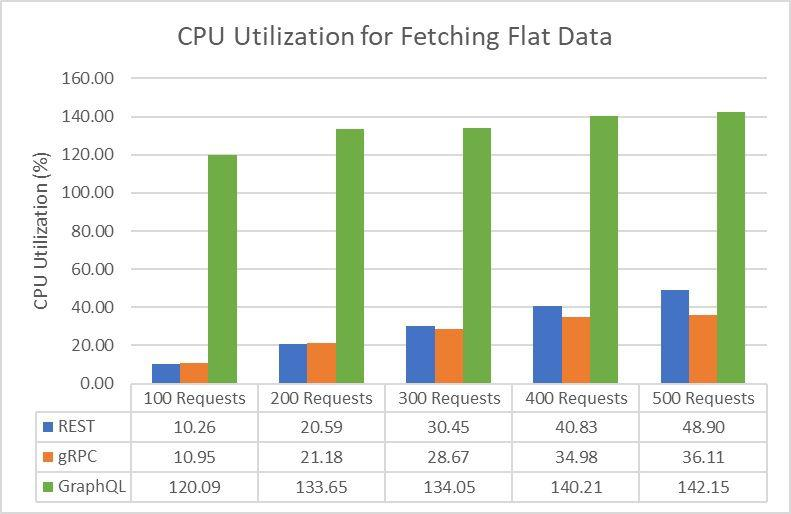
\includegraphics[width=\linewidth]{imagens/niswar_cpu_flat.jpg}    
    {\par \raggedright \footnotesize Fonte: \textcite{niswar_performance_2024}.\par}
  \end{minipage}%
  \hfill
  \begin{minipage}[t]{0.48\linewidth}
    \caption{Uso de CPU dos microsserviços com dados Aninhados}
    \label{fig:2-niswar-cpu-nested}
    \centering
    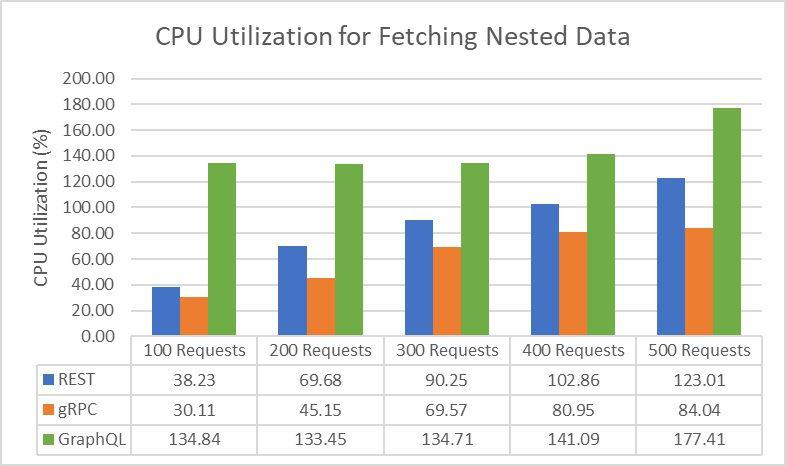
\includegraphics[width=\linewidth]{imagens/niswar_cpu_nested.jpg}    
    {\par \raggedright \footnotesize Fonte: \textcite{niswar_performance_2024}.\par}
  \end{minipage}
\end{figure}

A avaliação de requisições consecutivas, realizada durante cinco minutos e variando de 100 a 500 requisições, corroborou os achados dos testes concorrentes. O \gls{grpc} manteve-se como o protocolo com o tempo de resposta mais rápido para ambos os tipos de dados (flat e aninhados), evidenciando consistência sob diferentes padrões de carga. A capacidade do \gls{grpc} de utilizar o protocolo \acrshort{http}/2, que apresenta recursos como multiplexação (que permite múltiplas requisições sobre uma única conexão) e serialização binária eficiente (Protocol Buffers), é destacada pelos autores como o principal fator de seu desempenho superior em comparação ao \gls{rest} e ao \acrshort{graphql}.

\subsubsection{Resumo do Estudo}

Em suma, o estudo de \cite{niswar_performance_2024} conclui que o \gls{grpc} supera o \gls{rest} e o \acrshort{graphql} em termos de tempo de resposta, configurando-se como a escolha mais eficiente para comunicação em microsserviços que demandam baixa latência. Por outro lado, o \gls{rest} demonstrou menor utilização da CPU em alguns cenários, o que pode ser um fator relevante em ambientes com restrições de recursos. Embora o \acrshort{graphql} ofereça flexibilidade na recuperação de dados, resulta em maior consumo de CPU e aumento no tempo de resposta. As descobertas proporcionam insights práticos para a escolha de protocolos de \gls{api} em ambientes de microsserviços, levando em consideração os requisitos específicos de cada caso de uso e carga de trabalho.